% Graphics for slide 8, in the order the PDF draws them.
\begin{tikzpicture}[remember picture, overlay, x=1bp, y=-1bp,
  shift={(current page.north west)}]
\path[fill=cFFFFFF] (0,0) rectangle (960,540);
\path[fill=cEE7628,even odd rule] (57.18,55.73) ..controls(57.96,55.73)and(58.6,56.37)..(58.6,57.15) --(58.6,85.5) ..controls(58.6,86.28)and(57.96,86.91)..(57.18,86.91) ..controls(56.4,86.91)and(55.76,86.28)..(55.76,85.5) --(55.76,57.15) ..controls(55.76,56.37)and(56.4,55.73)..(57.18,55.73);
\node[anchor=north west, inner sep=0pt] at (68.12,107.55) {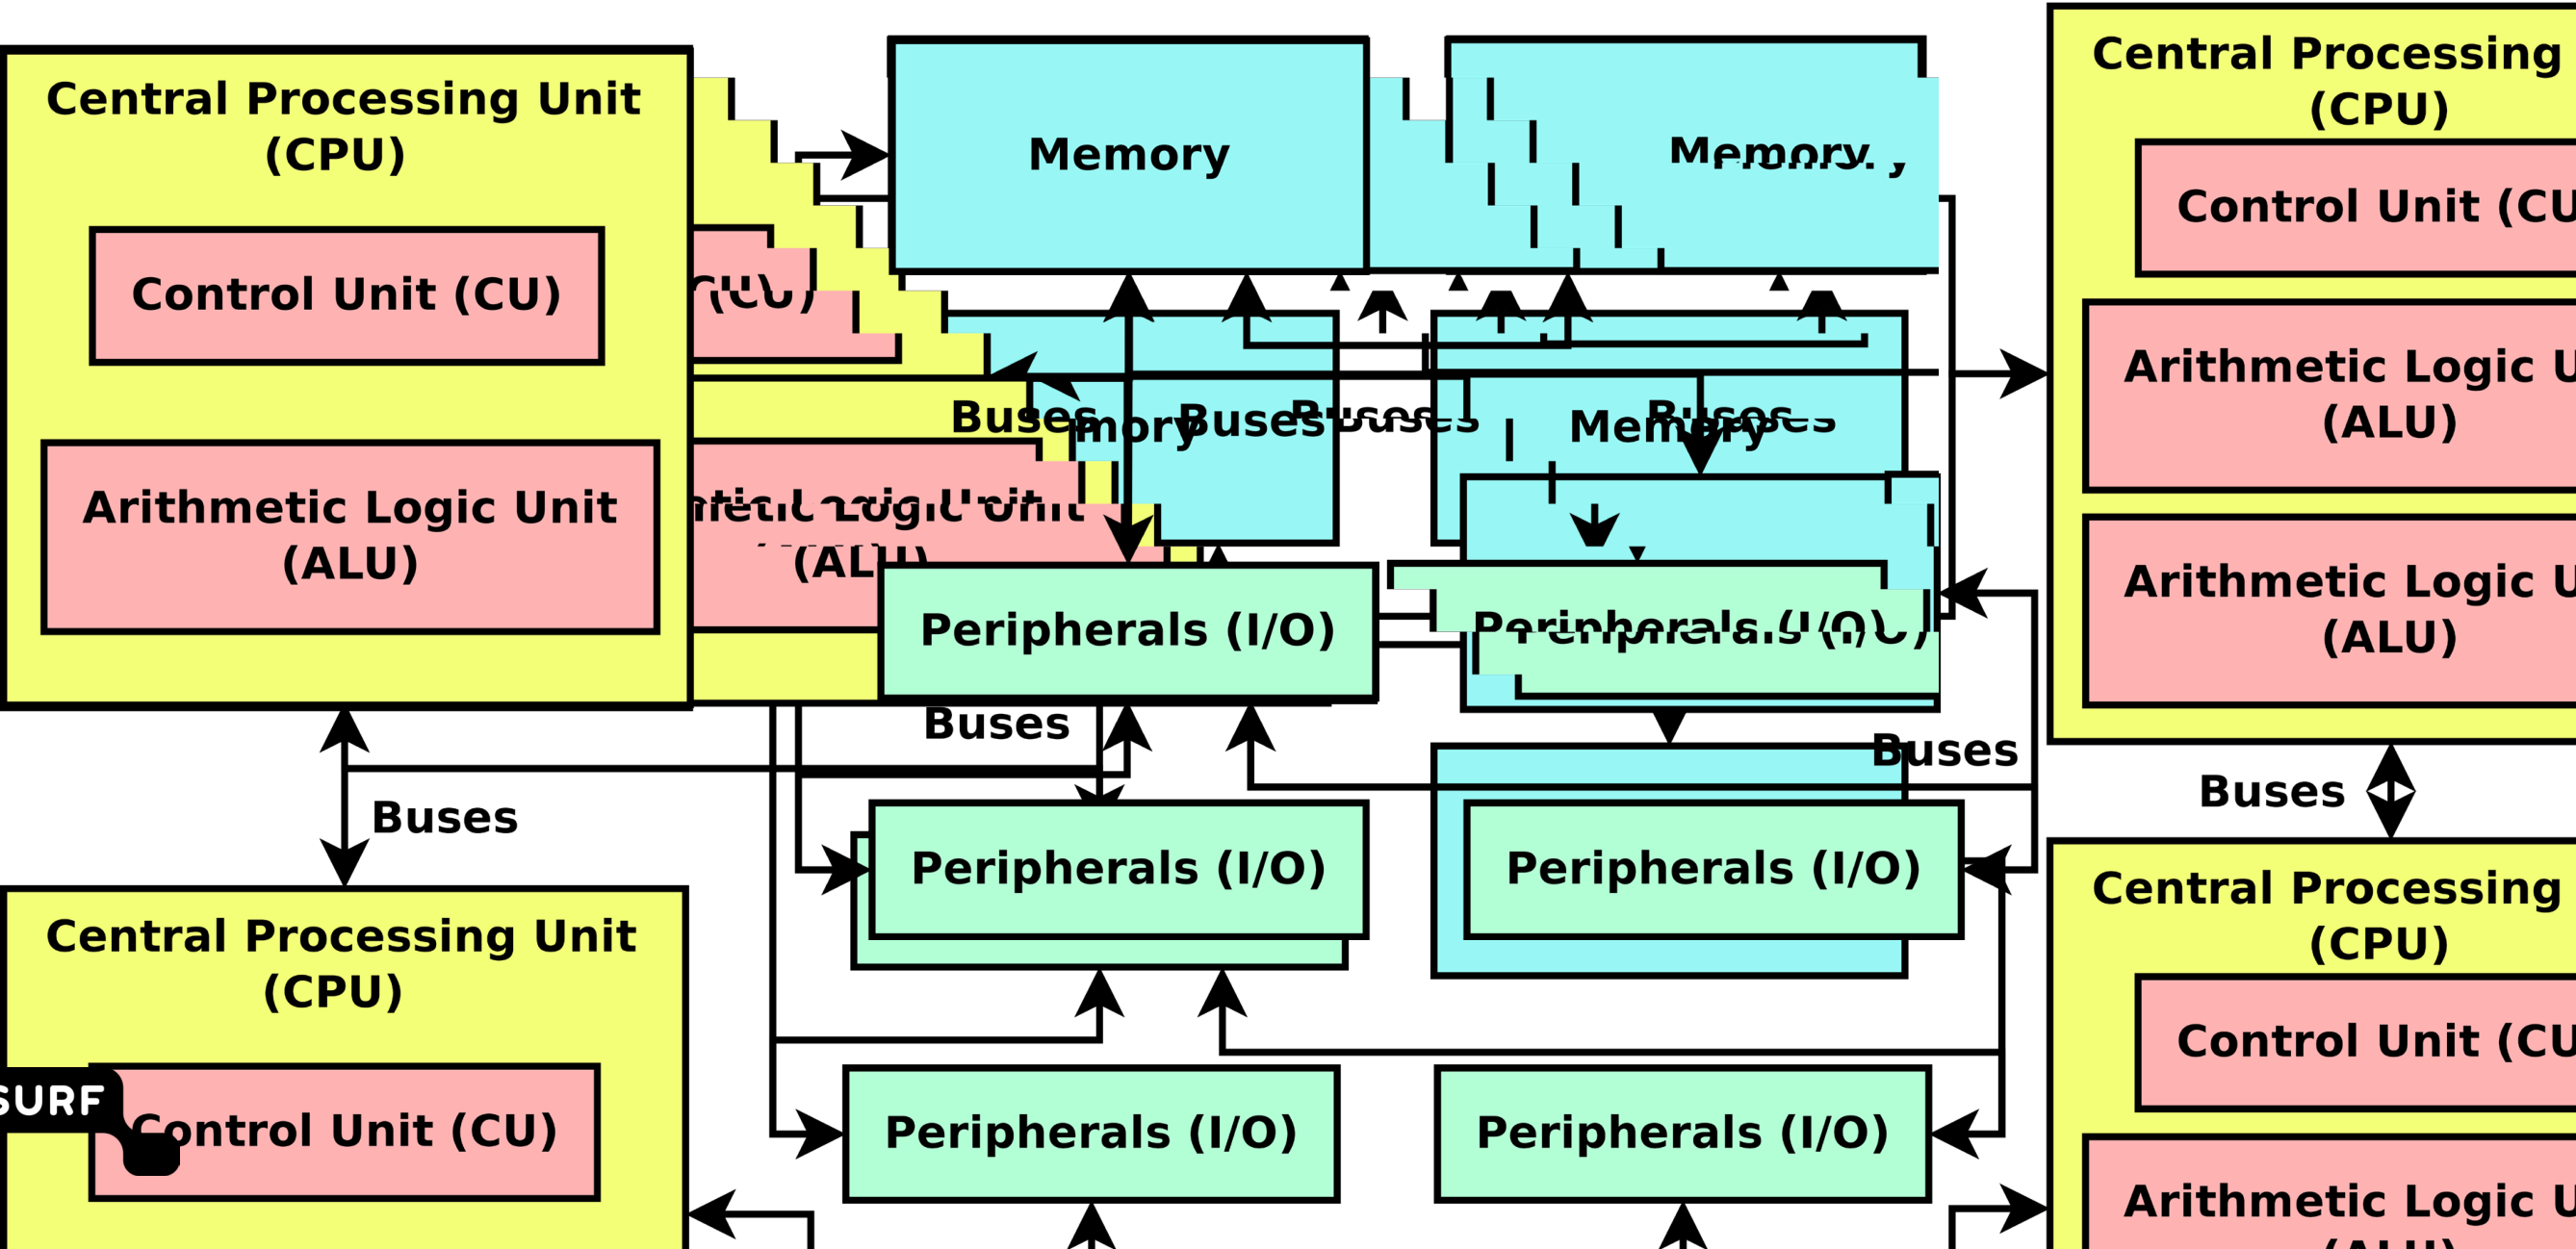
\includegraphics[width=891.88bp, height=432.45bp]{figures/fundamentals-of-hpc/p08-1.png}};
\node[anchor=north west, inner sep=0pt] at (68.12,119.51) {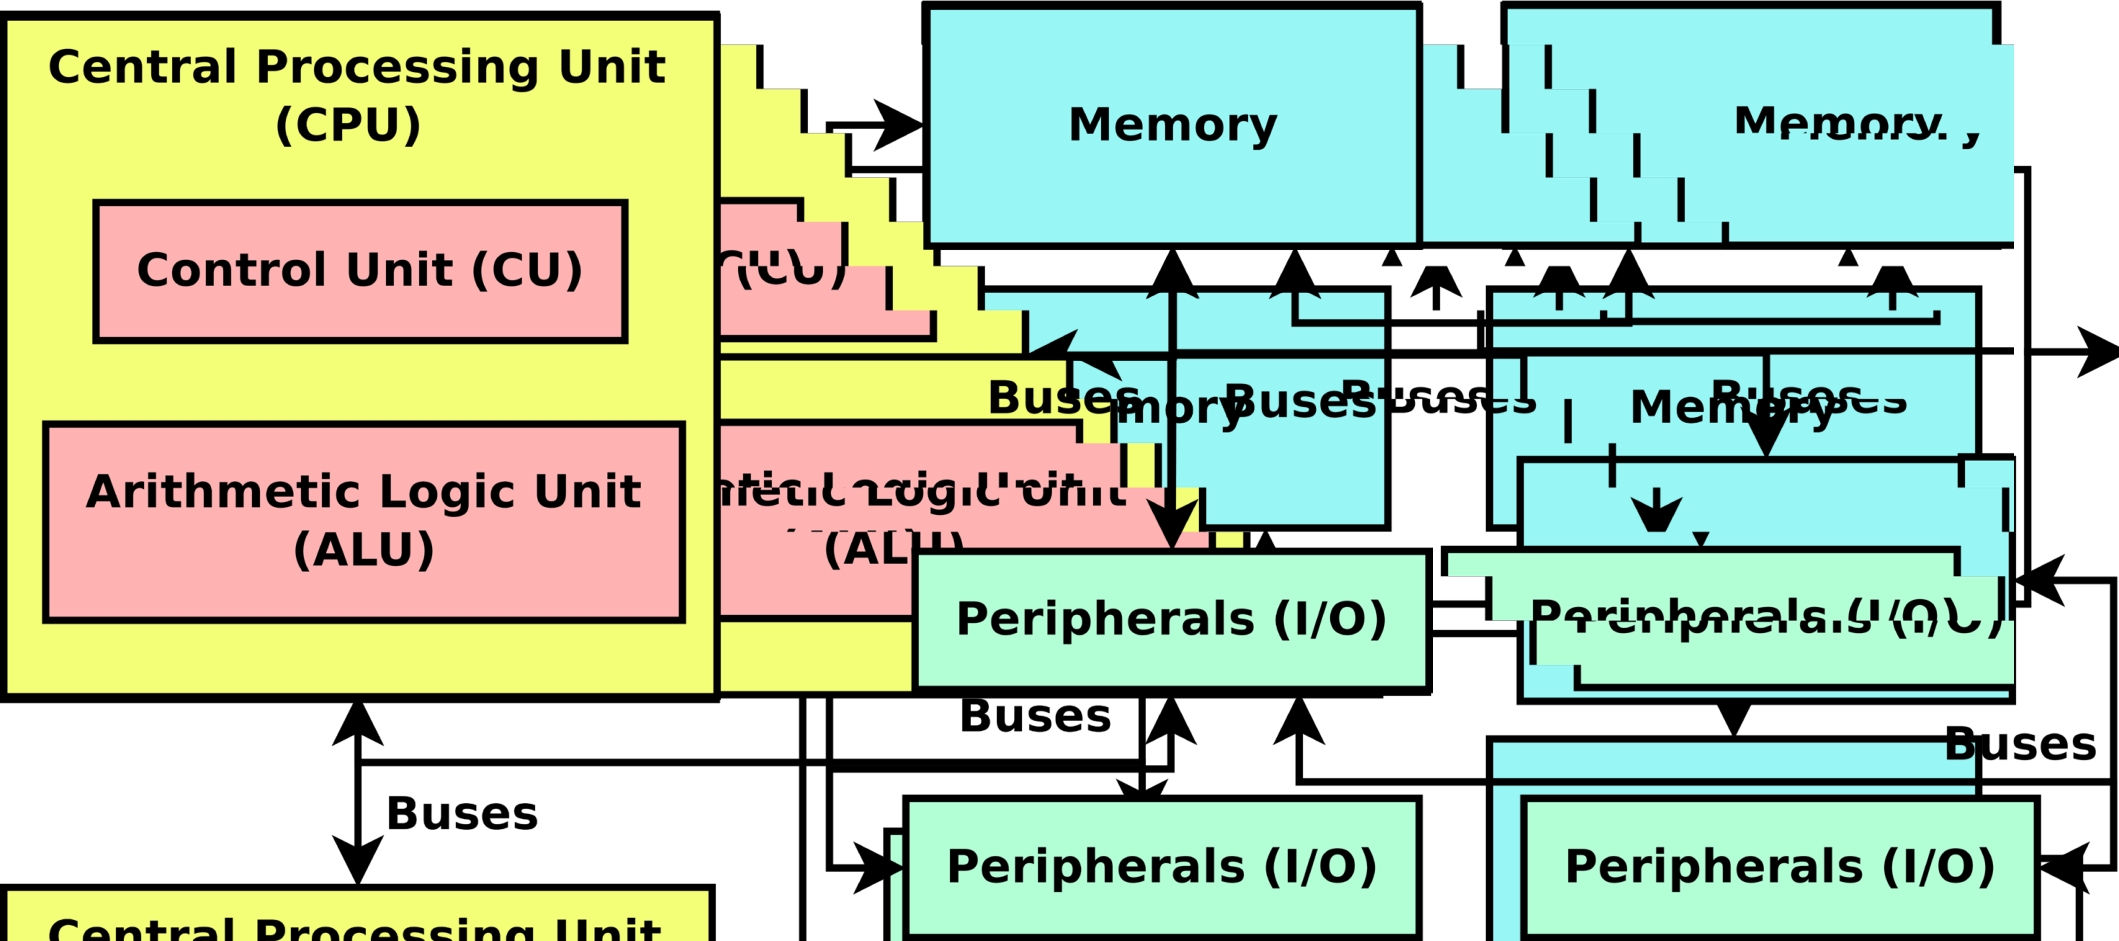
\includegraphics[width=706.06bp, height=313.21bp]{figures/fundamentals-of-hpc/p08-2.png}};
\node[anchor=north west, inner sep=0pt] at (68.12,119.51) {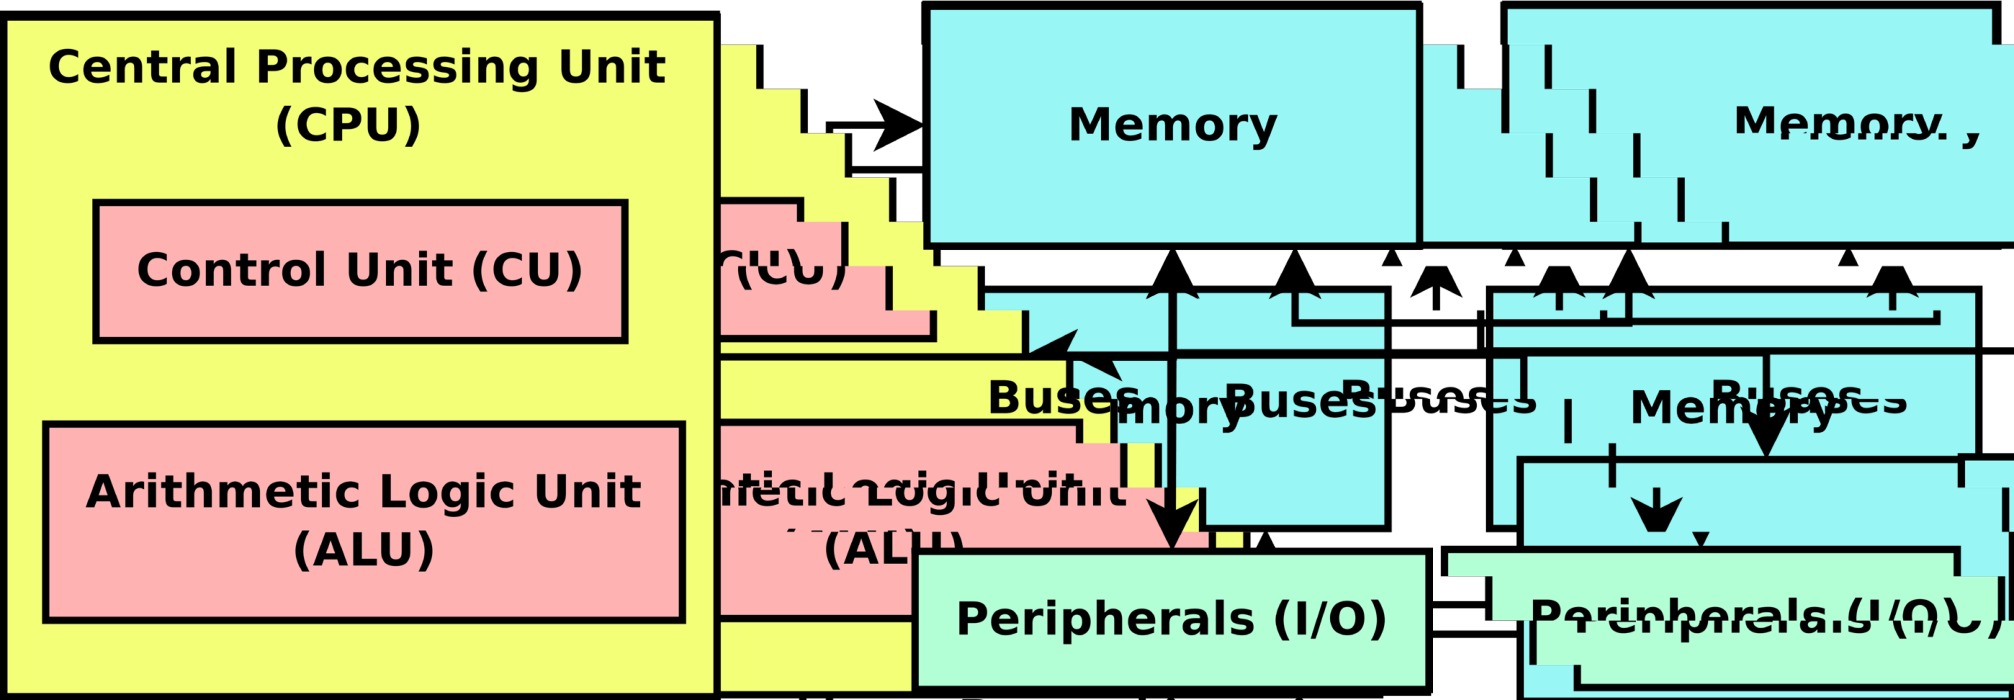
\includegraphics[width=671.11bp, height=233.13bp]{figures/fundamentals-of-hpc/p08-3.png}};
\node[anchor=north west, inner sep=0pt] at (68.12,119.51) {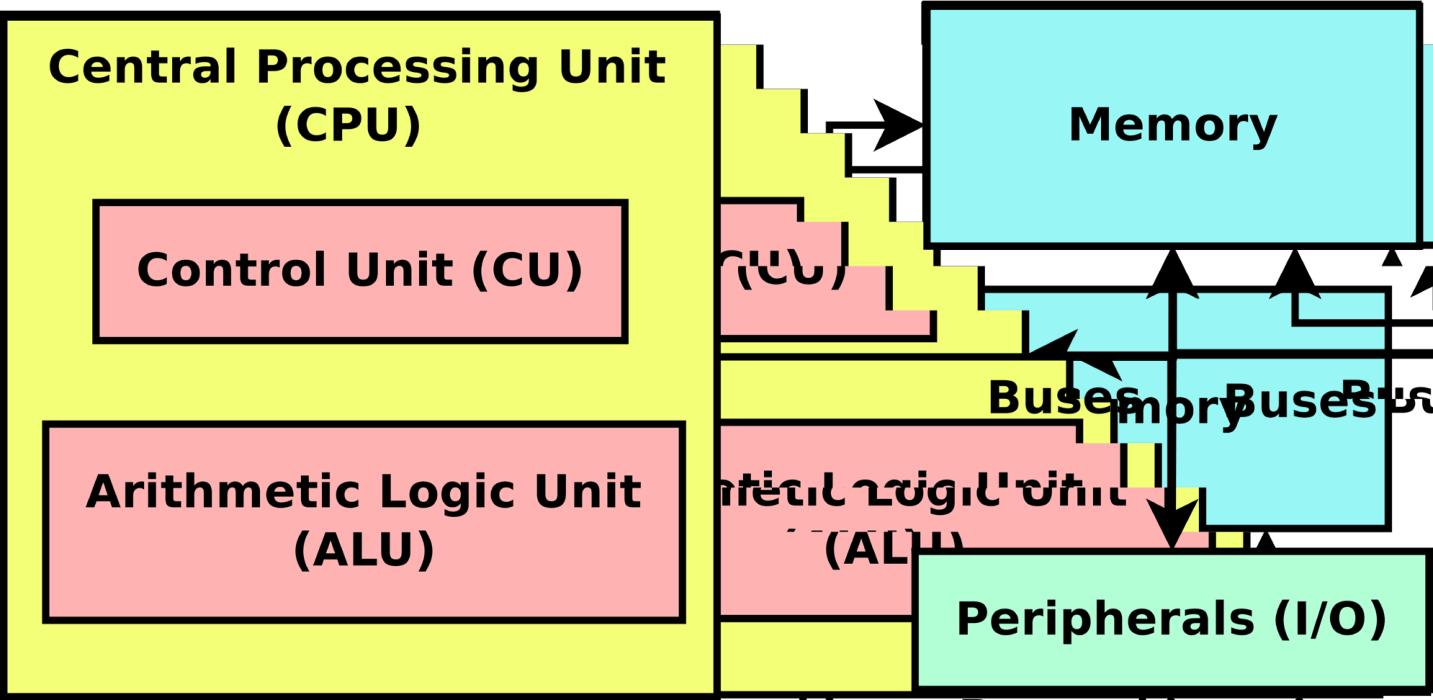
\includegraphics[width=477.44bp, height=233.13bp]{figures/fundamentals-of-hpc/p08-4.png}};
\node[anchor=north west, inner sep=0pt] at (56.69,477.21) {
\includegraphics[width=73.42bp, height=37.42bp]{figures/fundamentals-of-hpc/p08-5.png}};
\end{tikzpicture}
